\subsection{An\'alisis de Tiempo de C\'omputo}
\label{subsec:exp4}
\begin{LaTeXdescription}
    \item[Objetivo] Analizar la complejidad temporal del m\'etodo.

    \item[Hip\'otesis] Proponemos que el tiempo de c\'omputo por iteraci\'on
        para una instancia y $\epsilon$ fijos ser\'a siempre el mismo para todo
        $\alpha$. Tambi\'en proponemos que el tiempo de c\'omputo por interación
        para $\epsilon$ fijo ser\'a el mismo para \textbf{toda instancia} (sin
        importar tama\~no, cantidad de ejes, etc).\\

    \item[Proposici\'on] De los experimentos previo hemos llegado a la
        conclusi\'on de que a mayor $\alpha$, mayor cantidad de iteraciones
        ser\'an necesarias para converger, lo cual implica inmediatamente un mayor tiempo
        de c\'omputo requerido. La pregunta ideal a responder ser\'ia ''cu\'anto
        tiempo'', pero
        tambi\'en concluimos previamente que la cantidad de iteraciones es
        dependiente (entre otros factores) de la instancia de entrada. Con lo
        cual, responder a esta pregunta en el contexto de este trabajo es
        imposible sin una cota te\'orica para la cantidad de
        iteraciones (que ni siquiera sabemos si existe). En cambio, lo que si podemos analizar es
        si el tiempo de c\'omputo \textbf{por iteraci\'on} es el mismo para toda
        instancia, sin importar el $\epsilon$\footnote{M\'as all\'a de para nuestros
        experimentos lo estemos dejando fijo.} o $\alpha$. Analizamos entonces
        si el tiempo por iteraci\'on var\'ia seg\'un
        la densidad de la instancia inicial, y a su vez si varía para distintos
        valores de $\alpha$.\\

    \item[M\'etodo de Experimentaci\'on] Tomamos 3 instancias de tama\~no
        mediano-grande, con una diferencia relativa de densidad entre ellas
        significativa, particularmente, las mismas del experimento anterior.
        Luego resolvemos cada instancia con PageRank 10 veces para $\alpha=0.0$;
        $0.1$; $0.2$; $\dots$; $0.9$\footnote{Totalizando un total de 300
        corridas del m\'etodo (10 corridas para 10 valores de $\alpha$ para 3
        instancias distintas).}.  Tomamos entonces para cada instancia y
        $\alpha$ fijos, el promedio de los tiempos de c\'omputo. Por \'ultimo,
        calculamos el tiempo de c\'omputo por iteraci\'on dividiendo este
        promedio por la cantidad de iteraciones totales que necesit\'o el
        m\'etodo para converger.\\

    \item[Resultados, an\'alisis y discusi\'on]
        Consideramos 2 enfoques para extraer conclusiones, el primero analiza el
        tiempo consumido por iteración por el método de la potencia para diferentes
        valores de $\alpha$. Nuestra conclusión es que el tiempo es constante ya que
        el valor de $\alpha$ no modifica la \texttt{densidad} de la matriz
        original(El algoritmo 1 de Kamvar multiplica usando la matriz original).
        Puede observarse en los gráficos \label{subfig:exp4_tiempo_iteracion} y
        \label{subfig:exp4_tiempo_iteracion_log} que el tiempo oscila en valores muy
        pequeños alrededor del promedio. Mas empíricamente, se tienen las
        métricas\footnote{Diferencia \%: 100*(max-min)/max.} del cuadro
        \ref{tbl:exp4_data_notredame}. Creemos que estas variaciones se deben al
        scheduler y a fenómenos de bajo nivel de las corridas de los
        experimentos. El segundo enfoque centra su atención en el tiempo por
        iteracion respecto a la densidad del grafo de conectividad presentado.
        Al contrario que nuestra hipótesis, la densidad(cantidad de ejes) del
        grafo de conectividad si altera el tiempo de cómputo por iteración,
        creemos que esto se debe a que el producto $Ax$ del algoritmo 1 de
        Kamvar, ve alterada la \texttt{cantidad de valores no nulos por fila},
        haciendo que el producto matriz-vector requiera mas cómputos. Este
        comportamiento puede verse en el gráfico \ref{subfig:exp4_den}, que
        compara el tiempo promedio consumido\footnote{Se utiliza el valor
        promedio del tiempo sobre todos los factores de navegación.} contra una
        medida de densidad del grafo\footnote{Se toma como métrica un cociente
        escalado entre la cantidad de aristas del gráfo y la cantidad de aristas
        de una \texttt{clique} de su misma cantidad de nodos.}.
\end{LaTeXdescription}


\begin{figure}[H]
    \centering
    \subfloat[][Tiempo por Iteraci\'on en funci\'on de $\alpha$. Escala lineal]{
        \label{subfig:exp4_tiempo_iteracion}
        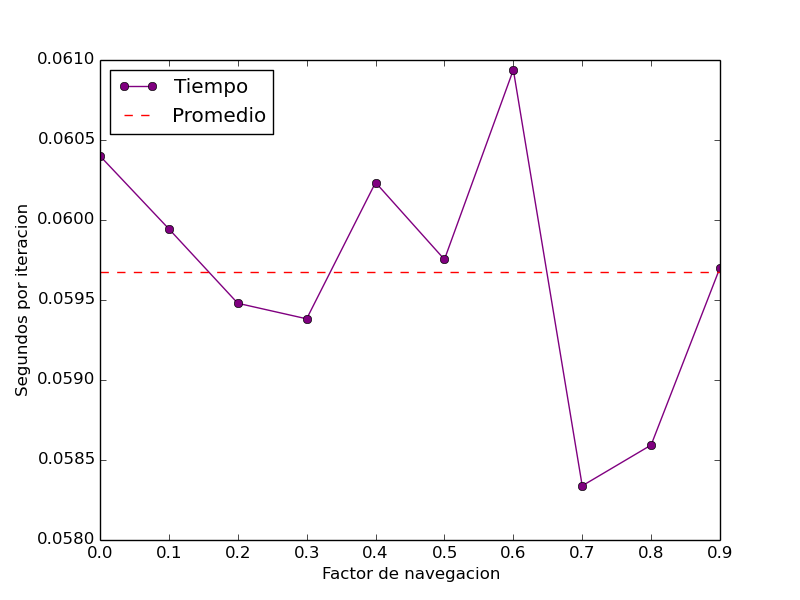
\includegraphics[width=.45\textwidth]{exp4_tiempo_por_iteracion_notredame.png}
    }
    \subfloat[][Tiempo por Iteraci\'on en funci\'on de $\alpha$. Escala logarítmica]{
        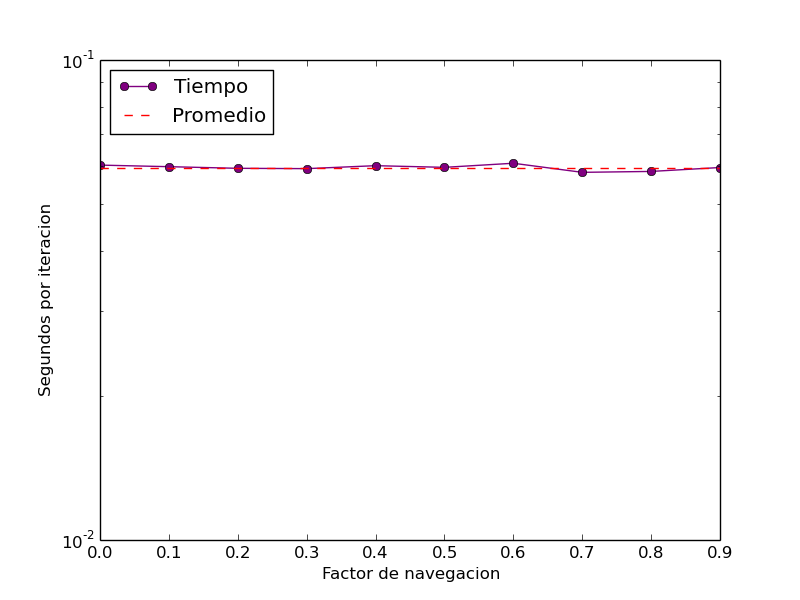
\includegraphics[width=.45\textwidth]{exp4_tiempo_por_iteracion_notredame_log.png}
        \label{subfig:exp4_tiempo_iteracion_log}
    }
    \caption{An\'alisis de Tiempo de C\'omputo en funci\'on de $\alpha$}
\end{figure}

\begin{table}[H]
    \centering
    \caption{Métricas acerca del tiempo por iteracion respecto de $\alpha$}    
        \label{tbl:exp4_data_notredame} 
    \setlength{\tabcolsep}{3pt}
    \begin{tabular}{|l|l|}
        \hline\hline
        Métrica & Valor(segundos)\\
        \hline
        Promedio & 0.059676\\
        Desv Estandar & 0.000788\\
        Min & 0.058338\\
        Max & 0.060938\\
        Diferencia \% & 4.266231\\
        \hline\hline
    \end{tabular}
\end{table}

\begin{figure}[H]
    \centering
    \subfloat[][Tiempo por Iteraci\'on promedio vs Densidad del Grafo]{
        \label{subfig:exp4_den}
        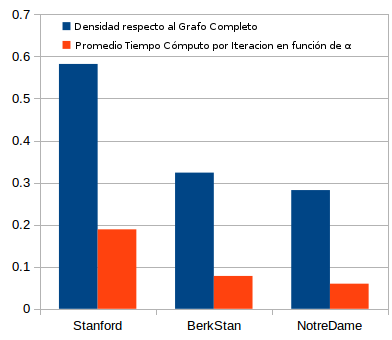
\includegraphics[width=.50\textwidth]{exp4_tiempo_vs_densidad.png}
    }
    \caption{An\'alisis de Tiempo de C\'omputo en funci\'on de la densidad del Grafo}
\end{figure}

    
